\chapter{Generalization error, Models, Hypothesis space}
\begin{chapquote}{A. Samuel}
    ``Machine learning is the science of getting computers to act without being explicitly programmed.''
\end{chapquote}

Machine learning is a very general and useful framework, but won't always work. In order to better understand when it will and when it will not work, it is useful to formalize the learning problem more.

\section{Task}
Tasks represent the type of prediction being made to solve a problem on some data. We can identify a task with the set of functions that can potentially solve it. In general, it consists of functions assigning each input \(x \in X\) an output \(y \in Y\).
\[f: X \to Y \qquad F_{\text{task}} \subset Y^X\]
The nature of \(X\), \(Y\) and \(F_{\text{task}}\) depends on the type of task.

\paragraph{Classification task}
The task for classification is to find a function \(f \in Y^X\) assigning each input \(x \in X\) a discrete label.
\[f(x) \in Y = \{c_1,...,c_k\}\]
Common classification applicaton are face recognition, character recognition, spam detection, medical diagnosis (from symptoms to illnesses), and biometrics.

\paragraph{Regression task}
The task for regression is to find a function \(f(x) \in Y\) assigning each input a \emph{countinuous} label.
Example of applications for regression task are in the field of economics/finance (predict the value of a stock), epidemiology, car/plane navigation (angle of the steering wheel, acceleration, ...), temporal trends (weather over time)..

\paragraph{Density estimation}
Density estimation is the construction of an estimate, based on observed data, of an unobservable underlying probability density function. The unobservable density function is thought of as the density according to which a large population is distributed.

The task for density estimation is to find a probability distribution \(f \in \Delta (X) \)\footnote{\(\Delta (X)\) is the set of all the probability distributions.} that fits the data \(x \in X\). 

\paragraph{Clustering task}
The task for clustering is to find a function \(f \in \mathbb{N}^X\) that assigns each input \(x \in X\) a cluster index \(f(x) \in \mathbb{N}\). All points mapped to the same index form a cluster.

Some applications for clustering tasks are social network analysis and genomics (group individuals by genetic similarity).

\paragraph{Dimensionality reduction task}
The task for dimensionality reduction is to find a function \(f \in Y^X\) mapping each (high dimensional) input \(x \in X\) to a lower dimensional embedding \(f(x) \in Y\), where \(\text{dim}(Y) \ll \text{dim}(X)\), and \(Y=\mathbb{R}^2\).

\section{Model and hypotesis space}
A \textbf{model} in machine learning is the output of a machine learning algorithm run on data. A model represents what was learned by a machine learning algorithm.

The model is the thing that is saved after running a machine learning algorithm on training data and represents the rules, numbers, and any other algorithm-specific data structures required to make predictions.

\begin{example}
    \begin{itemize}
        \item
        The linear regression algorithm results in a model comprised of a vector of coefficients with specific values.
        \item
        The decision tree algorithm results in a model comprised of a tree of if-then statements with specific values.
        \item
        The neural network/backpropagation/gradient descent algorithm together results in a model comprised of a graph structure with vectors or matrices of weigths with specific values.
    \end{itemize}
\end{example}

A machine learning model is more challenging for a beginner because there is not a clear analogy with other algorithms in computer science. The best analogy is to think of the machine learning model as a program, comprised of both data and a procedure for using the data to make a prediction. It is the implementation of a function \(f \in F_{\text{task}}\) that can be computed. The function \(f\) is an abstract concept, and the  model is the implementation.

We assume that the set of all possible model is a subset \(H \subset F_{\text{task}}\), called \emph{hypotesis space}.

\begin{example}[Polynomial curve fitting]
    \begin{center}
        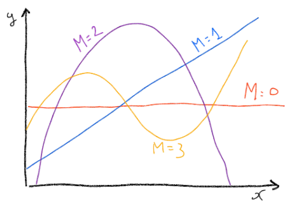
\includegraphics[width=0.4\textwidth]{018}
    \end{center}
    Data are the dots in the graph, and we want to learn the function. One way is to find the set of functions \(f\) and parametrize them with paremeter \(w\), multiplying with associated \(x\) to the power of \(j\). This corresponds to a polynomial of different degrees. 
    
    Model:
    \[f_w(x)= \sum_{j=0}^{M} w_jx^j\]
    Hypothesis space:
    \[H_M=\{f_w:w\in \mathbb{R}^M\}\]
    where \(H_M\) is the hypotesis space for fixed \(w \in \mathbb{N}\).
\end{example}

\subsection{The ideal target}
\begin{wrapfigure}{l}{0.35\textwidth}
\begin{center}
    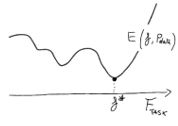
\includegraphics[width=0.35\textwidth]{019}
\end{center}
\label{fig:019}
\end{wrapfigure}
We want to minimize a generalization error function \(E(f;p_{\text{data}})\). The error function determines how well a solution \(f \in F_{\text{task}}\) fits some given data and guides the selection of the best solution in \(F_{\text{task}}\):
\[f^* \in arg\ \min_{f \in F_\text{task}} E(f; p_{\text{data}})\]

An error function tells how well my model fits some given data. Allows us to find the best \(f^*\) in the space of \(F_{\text{task}}\). Since this search space is too large and we do not have access to \(p_{\text{data}}\), we cannot complete this search, so we need an implementation for the error function.

\subsection{The feasible target}
\begin{wrapfigure}{l}{0.35\textwidth}
\begin{center}
    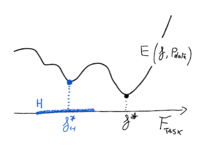
\includegraphics[width=0.35\textwidth]{020}
\end{center}
\label{fig:020}
\end{wrapfigure}
We need to restrict the focus on finding functions that can be implemented and evaluated in a tractable way. Thus we define a model and an hypotesis space \(H \subset F_{\text{task}}\) and seek a solution within that space.
\[f^*_H \in arg\ \min_{f\in H} E(f; p_{\text{data}})\]
We have restricted our search space, however we still may have some trouble computing the search, because \(p_{\text{data}}\) is unknown.

\subsection{The actual target}
\begin{wrapfigure}{l}{0.35\textwidth}
\begin{center}
    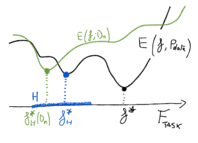
\includegraphics[width=0.35\textwidth]{021}
\end{center}
\label{fig:021}
\end{wrapfigure}
We need to revisit our minimization problem. Instead of using \(p_{\text{data}}\) we need to work on a data sample, i.e. a training set \(D_n=\{z_1,...,z_n\}\) where \(z_i=(x_i,y_i) \in X \times Y\), and \(z_i \sim p_{\text{data}}\).
\[f^*_H(D_n) \in arg\ \min_{f \in H} E(f; D_n)\]
This function is called training error and it does not match with the generalization error.

\section{Error function}
Machine learning can be thought of as an optimization problem, where there is an objective function that needs to be either maximized or minimized, and the best solution is the model that achieves either the highest or lowest score respectively. 

Typically in machine learning problems, we seek to minimize the error between the predicted value vs the actual value. The word \emph{error} represents the penalty of failing to achieve the expected output. If the loss is calculated for a single training example, it is called or \textbf{error function}. If the same loss is averaged across the entire training sample, the loss is called cost function.

Error function vary with the type of problem we are trying to solve. Regression problems that attempt to predict a continuous value have one set of loss functions, while the classification problems where the algorithm attempts to classify the training example into one of the target classes have another set of error/cost function.

Typically, the generalization and training error function can be written in terms of a pointwise loss \(l(f; z)\) measuring the error incurred by \(f\) on the training example \(z\).

\begin{align}
    &E(f; p_{\text{data}}) = E_{z \sim p_{\text{data}}}[l(f;z)]\\
    &E(f;D_n) = \frac 1 n \sum^n_{i=1}l(f;z_i)
\end{align}

\begin{figure}[h]

\label{fig:022}
\end{figure}
\begin{example}[Polynomial curve fitting]
\begin{center}
    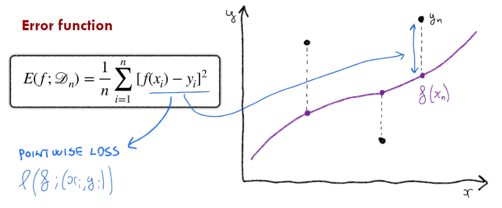
\includegraphics[width=0.6\textwidth]{022}
\end{center}
The pointwise loss is computed on each sample \(x_i\) separately. In this case it makes sense to have the square term, in this way we have the so called \emph{square loss}. Given our training data, we compute \(y_i\) and our function \(f\). Our objective is:
\[f^*_{H_M}(D_n) \in arg\ \min_{f \in H_M} E(f;D_n)\]
The objective is equivalent to \(f_{w^*}\), where \(w^*\) is defined as follows:
\[w^* \in arg\ \min_{w \in \mathbb{R}^M} \frac 1 n \sum^n_{i=1} [f_w(x_i)-y_i]^2\]
This requires to solve a linear system of equations.

\end{example}

Our learning algorithm solves the optimization problem targeting \(f_H^*(D_n)\), but might end up in a different result.
\begin{figure}[h]
\begin{center}
    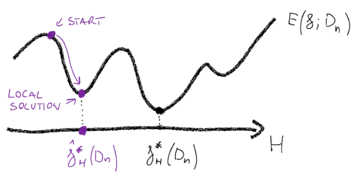
\includegraphics[width=0.5\textwidth]{023}
    \caption{}
    \label{fig:023}
\end{center}
\end{figure}

Let us put all the charts together, and build a recap chart for the \(f^*(D_n)\) function, showing the training error and the generalization error.
% TODO: add to summary
% \begin{figure}[h]
% \begin{center}
%     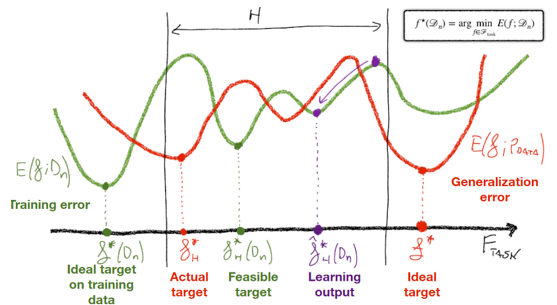
\includegraphics[width=0.75\textwidth]{024}
%     \caption{}
%     \label{fig:024}
% \end{center}
% \end{figure}

After performing our search, we obtain our learning output, this could introduce two potential problems, overfitting and underfitting.
\begin{figure}[h]
\begin{center}
    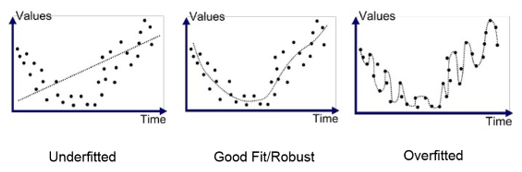
\includegraphics[width=0.75\textwidth]{025}
    \caption{Graphical representation of curve fitting}
\end{center}
\end{figure}

\subsection{Overfitting}
\textbf{Overfitting} is the production of an analysis that corresponds too closely or exactly to a particular set of data, and may therefore fail to fit additional data or predict future observations reliably.

An overfitted model is a statistical model that contains more parameters than can be justified by the data. The essence of overfitting is to have unknowningly extracted some of the residual variatione (i.e., the noise) as if the variation represented underlying model structure.

Overfitting occurs when the learned function \(\Hat{f}_H^*\), becomes sensitive to the noise in the sample. As the result, the function will perform well on the training set but not perform well on other data from the joint probability distribution of \(x\) and \(y\). Thus, the more overfitting occurs, the larger the generalization error.

\subsection{Underfitting}
\textbf{Underfitting} occurs when a machine learning algorithm cannot adequately capture the underlying structure of the data. It occurs when the model or algorithm shows low variance but high bias. It is often a result of an excessively simple model which is not able to process the complexity of the problem. This results in a model which is not suitable to handle all the signal and is therefore orced to take some signal as noise. 

If instead a model is capable to handle the signal but anyways takes a part of it as noise as well, it is also considered to be underfitted. The latter case can happen if the loss function of a model includes a penalty which is too high in that specific case.

An underfitted model would ignore some important replicable structure in the data and thus fail to identify effects that were actually supported by the data. In this case, bias in the parameter estimators is often substantial, and the sampling variance is underestimated, both factors resulting in poor confidence interval coverage. Underfitted models tend to miss important treatment effects in experimental settings.

\subsection{Estimate the generalization error}
The generalization error cannot be computed for \(p_{\text{data}}\), because it's unknown. The only possible way to access generalization error is by sampling. We use a data sample, and we assume that the probability distribution is the same for the training set, for the validation set, and for the test set.

We use the training set to find the best model, then the validation set to find the best hyperparameters. Once we have done this operation, we may think of having a way to estimate the generalization error in order to understand if the model will work well on the test data.

\begin{example}[Polynomial curve fitting]
\begin{center}
    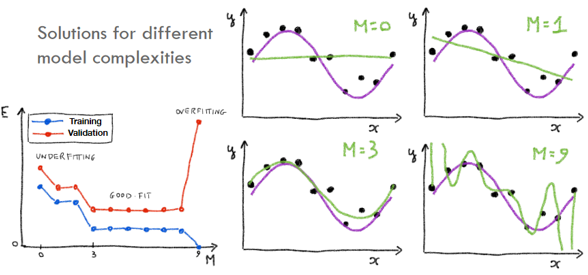
\includegraphics[width=0.75\textwidth]{026}
    \label{fig:026}
\end{center}
With the first model in Figure~\ref{fig:026}, there is an underfitting, high error, low performance in training and validation set. On the other side, with the last model there is overfitting, we approximate with almost 0 errors on training data, while performing poorly on unknown test data represented by smooth curve.

\end{example}

\subsection{Improve the generalization}
In order to improve generalization well, one needs to avoid both underfitting of the training data and overfitting of the training data.

There are a number of approeaches for improving generalization, one can:
\begin{itemize}
    \item
    Avoid to obtain the minimum on training error;
    \item
    Reduce the model capacity;
    \item
    Change the objective with a regularization term;
    \item
    Inject noise in the learning algorithm to smooth out the data points;
    \item
    Stop the learning algorithm before the convergence to avoid the model to learn too well on training data.
\end{itemize}

\subsubsection{Regularization}
The regularization is the modification of the training error function with a term \(\Omega(f)\) that typically penalizes complex solutions.
\[E_{\text{reg}}(f;D_n) = E(f;D_n) + \lambda_n \Omega (f)\]
We are adding another function \(\Omega\) to force the algorithm to learn a model with low complexity. It penalizes complex solution to find a simpler one, which can find a model that generalizes better (so to find a better \(f^*\)). The \(\lambda_n\) is a trade-off parameter.

\begin{example}[Polynomial curve fitting]
We regularize by penalizing polynomials with large coefficients:
\[E_{\text{reg}}(f;D_n) = \frac 1 n \sum_{i=1}^n [f_w(x_i)-y_i]^2 + \frac \lambda n ||w||^2\]
\[||w||^2 = \sum_i=w_i^2\]
We invoke norm regularization and set lambda hyperparameters by considering performance on validation set. The lambda parameter regulates the trade-off between underfitting and overfitting

% \begin{figure}[t!]
%     \begin{center}
%         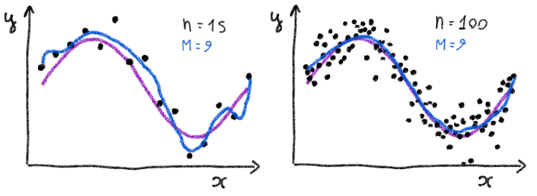
\includegraphics[width=0.75\textwidth]{028}
%         \caption{Generalization vs. data size for the polynomial curve fitting.}
%         \label{fig:028}
%     \end{center}
% \end{figure}

% \begin{figure}[h]
% \begin{center}
%     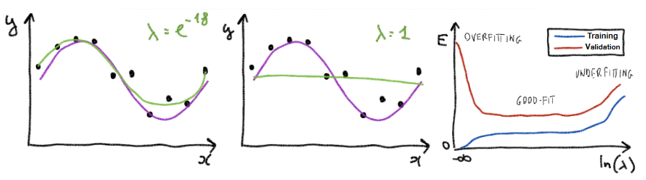
\includegraphics[width=0.75\textwidth]{027}
%     \caption{}
%     \label{fig:027}
% \end{center}
% \end{figure}

\end{example}

There are other approaches one can attempt, for example:
\begin{itemize}
    \item
    Increase the amount of data;
    \item
    Add more training samples;
    \item
    Augment the training set with transformations, when the provious is not possible;
    \item
    Combine prediction from multiple, decorrelated models to have preditions that are independent, and merging them we will probably get better labels. This technique is called \emph{ensembling}.
\end{itemize}

\begin{example}[Polynomial curve fitting]
Let's see the modification of the generalization in respect to the data size.
\[E(f;D_n) \to E(f;p_{\text{data}}) \qquad \text{as } n \to \infty\]
A graphical representation is provided in Figure~\ref{fig:028}.

\begin{center}
    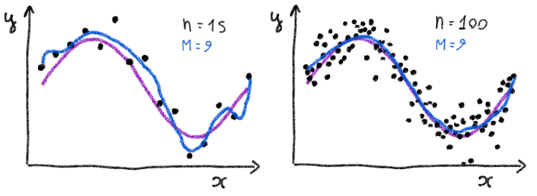
\includegraphics[width=0.75\textwidth]{028}
    \label{fig:028}
\end{center}
\end{example}

\newpage
\begin{exercise}[topsep=20pt, itemsep=10pt]
\end{exercise}